

\documentclass[conference]{IEEEtran}
\IEEEoverridecommandlockouts
\usepackage{blindtext, graphicx}
\usepackage{subfigure}
\usepackage{booktabs}
\usepackage{array}
\usepackage{cite}
\usepackage{makecell}
\usepackage{enumerate}
\usepackage{caption}
\usepackage{amsmath}
\usepackage{multirow}
\usepackage{tikz}
\usepackage{breqn}
\usepackage{algorithm}

\usepackage{algpseudocode}
\usepackage{pifont}

\usepackage{mathtools}
\usepackage{url}




\makeatletter
%%%%%%%%%%%%%%%%%%%%%%%%%%%%%% User specified LaTeX commands.
\def\ps@IEEEtitlepagestyle{%
  \def\@oddfoot{\mycopyrightnotice}%
  \def\@evenfoot{}%
}
\def\mycopyrightnotice{%
  {\footnotesize 978-1-4673-9044-6/16/\$31.00  \copyright 2016 IEEE\hfill}
  \gdef\mycopyrightnotice{}% just in case
}

\usetikzlibrary{shapes.geometric, arrows,calc,fit}
\tikzset{box/.style={draw, rectangle, rounded corners, thick, node distance=7em, text width=6em, text centered, minimum height=3.5em}}
\tikzset{container/.style={draw, rectangle, dashed, inner sep=2em}}
\tikzset{line/.style={draw, thick, -latex'}}
\ifCLASSINFOpdf
 
 \else
 \fi
% correct bad hyphenation here
\hyphenation{op-tical net-works semi-conduc-tor}


\begin{document}
%
% paper title
% can use linebreaks \\ within to get better formatting as desired
\title{A Novel Decision-Making Mechanism of  Resource Scheduling in High-Speed Trains in Push-based Wireless Converged  Broadcasting and Cellular Networks }


% author names and affiliations
% use a multiple column layout for up to three different
% affiliations
%\author{
%\IEEEauthorblockN{Xia Li}
%\IEEEauthorblockA{Department of Electronic Engineering\\
%Shanghai Jiao Tong University\\
%Shanghai, China\\
%Email: lixia19920625@gmail.com}
%}

\author{\IEEEauthorblockN{Bing Li\IEEEauthorrefmark{1}, Jian Xiong\IEEEauthorrefmark{2}, IEEE Member, Bo Liu\IEEEauthorrefmark{2}, IEEE Member, Lin Gui\IEEEauthorrefmark{2}, IEEE Member \\and Meikang Qiu\IEEEauthorrefmark{3}, Senior IEEE Member}\\
\IEEEauthorblockA{\IEEEauthorrefmark{1}\IEEEauthorrefmark{2}Department of Electronic Engineering, Shanghai Jiao Tong University, Shanghai, China\\
\IEEEauthorblockA{\IEEEauthorrefmark{3}Department of Computer Science, Pace University, New York City, USA.}
\IEEEauthorrefmark{1}Email: libing0826@hotmail.com\\
\IEEEauthorrefmark{2}Email: \{xjarrow, liubo\_lb, guilin\}@sjtu.edu.cn\\
\IEEEauthorrefmark{3}Email: mqiu@pace.edu
}
}

% make the title area
\maketitle


\begin{abstract}
%\boldmath
%
%In this paper, we maximize the network capacity and alleviate request congestion by forward pushing the most popular multimedia contents through broadcasting/multicasting, and on the user side locally caching for further request. In the proposed model, based on a converged broadcast and cellular network, we present a content distribution scheme in wireless cellular networks and a corresponding scheduling algorithm. Furthermore, to improve user experience and meet the demands of various users, we propose a sleep-awake scheme and UE-based cache replacement algorithms with user equipment forward caching popular contents. Simulations show that the proposed algorithms can significantly reduce the network resources consumption including boosting the capacity of the traditional cellular network and increasing the network throughput efficiency. Moreover, on the user side we compare the performance between the proposed architecture and the traditional cellular network, and the result shows that the proposed scheme can bring improvements on energy saving. 


% Proxy server in base station (\emph{BS}) schedules the popularity-ranked contents and transmits them to all users by Point to Multi-Point (\emph{P2M}) mode, and user equipments (\emph{UEs}) locally cache those contents. when users request for a specific content, the target is most likely cached (\emph{cache hit}) due to \emph{Matthew Effect}. %Evolved Multimedia Broadcast Multicast Services (\emph{eMBMS}) in LTE standards provides a scheme to implement Point to Multi-Point transmission.

Int this paper, we propose a novel decision-making mechanism  of Resource Scheduling (RS) in high-speed trains in the push-based Wireless Converged  Broadcast  and  Cellular  Network (WCBCN) . In this model, we transform dynamic programming problem into the static issue. When the train set out from the origin station, the WCBCN start to broadcast the hot-spot information which have been already downloaded at the Cloud Computing Center (CCC) to all passengers in the trains.Because there will be some passengers on or off the train in the next railway station. In order to maximize the capacity of the WCBCN, the CCC will decide whether to 
 retransfer the most popular contents or not before the train set out from the next station.  It's intuitive  that the capacity will improve to some extent.
 Simulations show that proposed model for the high-speed mobile environment can increase the capacity by 50\%-60\% comparing with the traditional one.  
\end{abstract} 

\begin{IEEEkeywords}
Wireless Converged Broadcast and Cellular Network (CWBCN), Cloud Computing Center (CCC),  High-speed train, information retransmission.
\end{IEEEkeywords}

\IEEEpeerreviewmaketitle

\section{Introduction }
Recently, more and more people choose the high-speed railway (HSR) as their means of transportation due to its Low-Carbon and time saving. Moreover, high-speed trains with a speed of 300 KM/h have been rapidly deployed all over the world\cite{380km}. While the popularity of portable equipments which support various multimedia contents, e.g., smartphones, ipad, have bring us into a big data time. Nowadays, information blows up  with the form of exponential growth. No matter where we are, most of us would like to get their interested contents including videos, files, audio from abundant contents providers through the mobile Internet.  

Under this situation, converged network, as single wireless network could no longer meet the demand of many scenarios, has become a focus recently. Previously a number of topics have been researched in the field of converged network, like Converged Broadcasting and Cellular Networks \emph{(CBCN)} based on DVB-H/DVB-T, DMB, ISDB-T, MediaFLO, etc, and in the undergoing research of 5G cellular technologies, Mobile broadcasting comes of age in LTE eMBMS(evolved Multimedia Broadcast Multicast Services),
eMBMS Provides Excellent Broadcast Performance, at present the application of LTE-broadcast(LTE-eMBMS) is with an efficient P2M(point to multi-point) distribution feature that can simultaneously serve many LTE-broadcast capable terminals with the same content. Based on this, LTE-broadcast can be used to boost network capacity for live or on-demand content such as top websites, breaking news or popular video which can be broadcast-offloading the network and providing users with a superior experience\cite{lohmar2013delivering}. 

However, under this circumstances, the existing application of converged network is more of a real time solution, which means the users are requesting for the same content at the same time. Based on statistical user trace, the massive requests are not randomly consumed on all contents. A number of researches have been done around the user request distribution\cite{cha2007tube}, indicating that there exists Matthew effect in those massive requested multimedia contents, and helping some contents gain popularity\cite{bastug2014living}. That is, a majority number of users are mainly requesting for a small part of contents, we name these contents \emph{popular contents}. To extend the limitation, we proposed a cache mechanism in the client (\emph{UE}) to cache the most popular contents so that equivalently the application can handle with users' requests asynchronously. Caching is widely used to improve user experience, alleviate request congestion and reduce resource consumption in communication networks. In the context of wireless communication networks, various caching schemes have been proposed, including base station caching, proxy caching, relay caching and client caching\cite{bao2012energy}. In \cite{peng2015backhaul}, the authors consider a wireless caching network where all the BSs are connected to a central
controller via backhaul links. In \cite{ahlehagh2014video}, the authors studied video caching in the radio access network and proposed caching policies based on the user preference profile.

While most of them take base station cache or relay cache more into account in existing researches, as most of user terminals have been updated to smartphones, and the local data storage have been lower-cost and faster-response, there are reasons to believe locally forward caching in user equipments would be a practicable solution. ``Local Forward Caching'' refers to a terminal saving a content forwardly, then reusing it later instead of re-requesting the same asset from the base station again. 
 
 
In this paper, to support the popular contents forward caching based on converged network, it is required to propose a content-pushing scheme and an efficient hybrid scheduling algorithm on \emph{UE} side and evaluate its performance.
 
The main contributions of this work can be summarized as follows:
\begin{itemize}
\setlength \itemindent {-1 em}
\item
Firstly, we introduce a UE-based cache replacement mechanism, in which we take both frequency and recency of popular services into consideration. Simulations show that the adopted algorithm in our architecture can significantly improve the capacity of the CWBCN.

\item
Then, based on the cache replacement mechanism, a sleep-awake algorithm of pushing process is proposed to reduce the energy consumption of UE. Simulations show that the performance of the proposed sleep-awake algorithm is further improved and far outweighs the traditional ones.
 \end{itemize}

The rest of the paper is organized as follows. In Section II, we discuss our system model which includes the analysis of the popularity distribution of user request, architecture of request and response scheme. Section III presents our problem formulation and the proposed algorithm. In Section IV, we evaluate our work by performance analysis. Section V concludes the paper. 
 

\section{System model}
%In this work, we consider a scenario:
\subsection{User Request Distribution}
Several research contributions on meeting the distribution of the popularity of requesting contents, like user generated content, video-on-demand\cite{cha2007tube}. Research shows that ZIPF's law provides an statistically accurate fit with these multimedia contents\cite{wang2014push}. To confirm the validity, we mine data on the real Internet traffic traces from one of the most popular Chinese portal sites, and the result is consistent with the zipf law.

\subsection{Converged Network with Popular Contents Forward Push}
Consider a single cell in a traditional cellular network, there are $N$ active users in the coverage, all of users send request for the contents to the same base station. For illustrative purposes, here gives a simple example, in a time slot, each user $i$ ($u_i$) send a request for content $j$ ($c_j$), let us denote the bandwidth of each subchannel as $B_{csi}$, the average bandwidth efficiency as $B_{cei}$ and assume there is no blocked request, as a result, the network capacity is $\sum_{i=1}^N {B_{csi}B_{cei}(bps/Hz)}$.

In the converged network with popular contents forward push, a popular contents set  $pc=\{m_1,m_2,m_3,...,m_k\}$ are forward pushed to each user through broadcasting, and locally cached by each user. Once the requested content $c_j \in pc$, we name it a cache hit event, and if the hit rate is $r_i$, that is, in this time slot, there are $r_i\lambda_i$ cache events occur, let us denote the broadcast bandwidth as $B_b$, and the average bandwidth efficiency as $B_{ce}$, then the equivalent network capacity is $\sum_{i=1}^N {B_{csi}B_{cei}} + r_i\lambda_i B_bB_{be}$. This is the prototype of our ideas.

\subsection{Base Station Controller Server \emph{(BSCS)}}
Web proxies and Content Distribution Networks are widely used to accelerate web content delivery and to conserve internet bandwidth. In our architecture, we add a layer between UE and basestation, called Base Station Controller Server, as a proxy server.
Traditional proxy servers are deployed by Internet Service Providers (\emph{ISPs}) to deal with increased Web traffic and optimize the content delivery on the Web.
Caching is widely used to improve user experience. ISPs use proxies to store the most frequently or most recently requested content\cite{stamos2008caching}. We innovatively proposed \emph{BSCS} to dynamically store and schedule the most popular contents for the UEs in the base station coverage area. The \emph{BSCS} preloads contents from \emph{ISPs} into its memory based on a set of predetermined popularity rank for future broadcast pushing.

%\subsection{Utility Function}
%Since the popular contents are \emph{forward} cached and users' requests cannot be accurately predicted, cache miss will always be there. For a user, cache miss will undoubtedly be a waste of resources, thus degrade the user experience. So the cache hit will save the network resource while cache miss is a waste of resources, here comes the trade-off. To numerically analyze how the cache hits/misses affect users' experience, we adopt a hit rate based utility function as a user's Quality of Experience(QoE)\cite{khan2011user}.

\subsection{Scenario}
Fig. \ref{scenario} is the scenario of this paper, in this architecture, on the station side, in addition to traditional cellular base station, there is a base station which serves multi-cell simultaneously by a \emph{BSCS}, it can automatically schedule its cache with \emph{ISP} and update the cache with upcoming popular contents. In the meantime, it polls popular contents to all the users in its region by broadcasting. On the user side, each \emph{UE} has its own cache for the broadcasting popular contents, to increase the flexibility and provide better scheme evolution, each \emph{UE}'s broadcasting channel can switch on or off autonomously.
  
%In this paper, we implement point to multipoint transmission by LTE-eMBMS rather than traditional broadcast network, with an BSCS in LTE base station. Multicast services can be transmitted in P2M mode within eMBMS areas. 
\begin{figure}[!h]
\centering
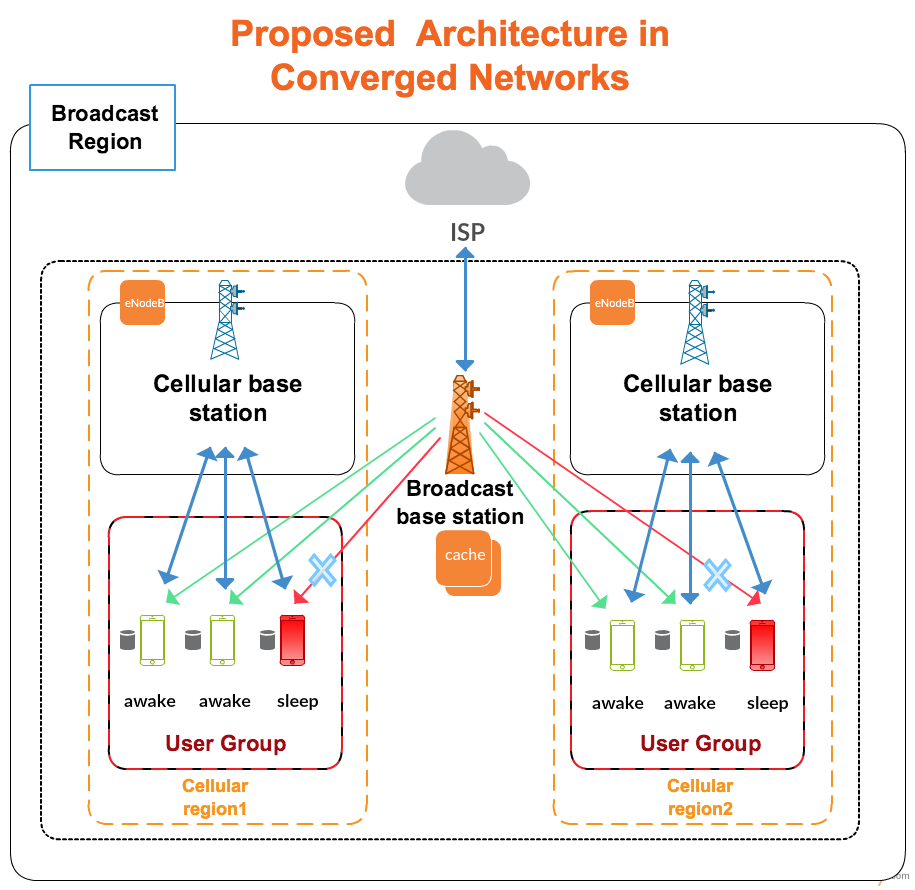
\includegraphics[width=8.8cm]{figure/converged.png}
 \caption{Proposed converged networks architecture}
\label{scenario}
\end{figure}
The request stream can be described as Fig \ref{Fig.1}: When a UE requests an Internet service, such as HTTP, the client checks its local cache for the data and, if the data is available, sends it to the client immediately. If the data is not available, the client requests the data from the hierarchical BSCS then base station requests to the origin ISP, and then returns the data to the client.



\begin{figure}[!hbt]
\centering
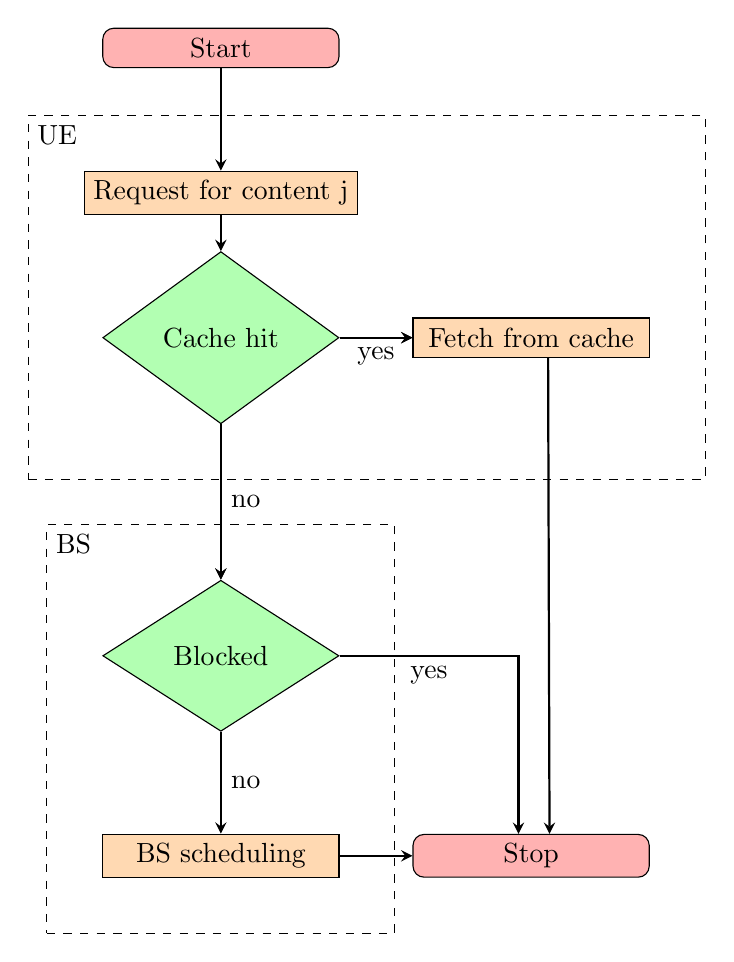
\begin{tikzpicture}[node distance=1.84cm]
\tikzstyle{startstop} = [rectangle, rounded corners, minimum width=3cm, minimum height=0.5cm,text centered, draw=black, fill=red!30]
\tikzstyle{io} = [trapezium, trapezium left angle=70, trapezium right angle=110, minimum width=3cm, minimum height=0.5cm, text centered, draw=black, fill=blue!30]
\tikzstyle{process} = [rectangle, minimum width=3cm, minimum height=0.5cm, text centered, draw=black, fill=orange!30]
\tikzstyle{decision} = [diamond, minimum width=3cm, minimum height=0.5cm, text centered, draw=black, fill=green!30]
\tikzstyle{arrow} = [thick,->,>=stealth]

\node (start) [startstop] {Start};
\node (req) [process, below of=start] {Request for content j};
\node (dec1) [decision, below of=req] {Cache hit};
\node (pro2a) [process, right of=dec1, xshift=2.1cm] {Fetch from cache};
\node (dec2) [decision, below of=dec1, yshift=-2.2cm] {Blocked};
\node (bs_sch)[process,below of=dec2,yshift=-0.7cm]{BS scheduling};
\node (stop) [startstop, right of=bs_sch,xshift=2.1cm] {Stop};

\node[container, fit=(req) (dec1)(pro2a)] (UE) {};
\node at (UE.north west) [above right,node distance=0 and 0, yshift=-0.5cm] {UE};
\node[container, fit=(dec2) (bs_sch)] (BS) {};
\node at (BS.north west) [above right,node distance=0 and 0, yshift=-0.5cm] {BS};

\draw [arrow] (start) -- (req);
\draw [arrow] (req) -- (dec1);
\draw [arrow] (dec1) -- (pro2a);
\draw [arrow] (dec1) -- (dec2);
\draw [arrow] (dec1) -- node[anchor=north]  {yes} (pro2a);
\draw [arrow] (dec1) -- node[anchor=west] {no} (dec2);
\draw [arrow] (dec2) -| node[near start][anchor=north] {yes} (stop.120);
\draw [arrow] (dec2) -- node[anchor=west] {no} (bs_sch);
\draw [arrow] (bs_sch) -- (stop);
\draw [arrow] (pro2a.310) --(stop.50);

\end{tikzpicture}
\caption{\label{Fig.1}BS to UE request stream} 
\end{figure}

\section{Problem Formulation and Algorithm}
In this section, basic definitions and key notations are first introduced, and provide a basic formulated model. Then the UE-based cache replacement algorithm and push strategy are described.
\begin{table}
\footnotesize
\renewcommand
\arraystretch{1}
\begin{center}
\caption{\label{Table1}definition of Parameters}
\begin{tabular}{c|c}
\toprule
\hline
   Parameter & Definition  \\
  \hline
$B_b$ & Broadcasting bandwidth \\
$B_{be}$ & Broadcasting bandwidth efficiency\\
$B_{cs}$ & Cellular subchannel bandwidth \\
$B_{ce}$ & Cellular subchannel bandwidth efficiency \\
$N$  & Number of users in one cell\\
$N_s$ & Num. of subchannels \\
$N_b$ & Num. of broadcasting contents \\
$N_{bmax}$ & Ceiling of broadcasting contents \\
$p_{ci}$ & Power consumption on cellular network \\
$p_{bi}$ & Power consumption on broadcasting network  \\
$r_i$   & Broadcasting hit rate of user $i$'s requests \\
$\xi_i$ & User $i$ cache size \\
$\zeta _0$ & Average size of content\\
 $\lambda_i$ & User $i$ requesting rate\\
$\eta$ & Throughput Efficiency\\
P & Allowed max power of a user for data transmission \\ 
  \hline
\bottomrule
\end{tabular}
\end{center}
\end{table}

\subsection{Problem Formulation}
The definitions of parameters shown in Table \ref{Table1}.

As described above, user request distribution follows zipf distribution, the probability density function of the zipf distribution is given by
\begin{equation}\label{zipf_pdf}
\begin{aligned}
pdf: f(j;z,N)=\frac{(1/j)^z}{\sum_{n=1}^N{(1/n)^z}}=\frac{1}{j^zH_{N,z}}
\end{aligned}
\end{equation}

%As a result, we can found that the cache hit rate will theoretically converge as the amount of contents increase, which is shown in Fig \ref{Fig.2}.
%%\begin{figure}[hbt]
%%\centering
%%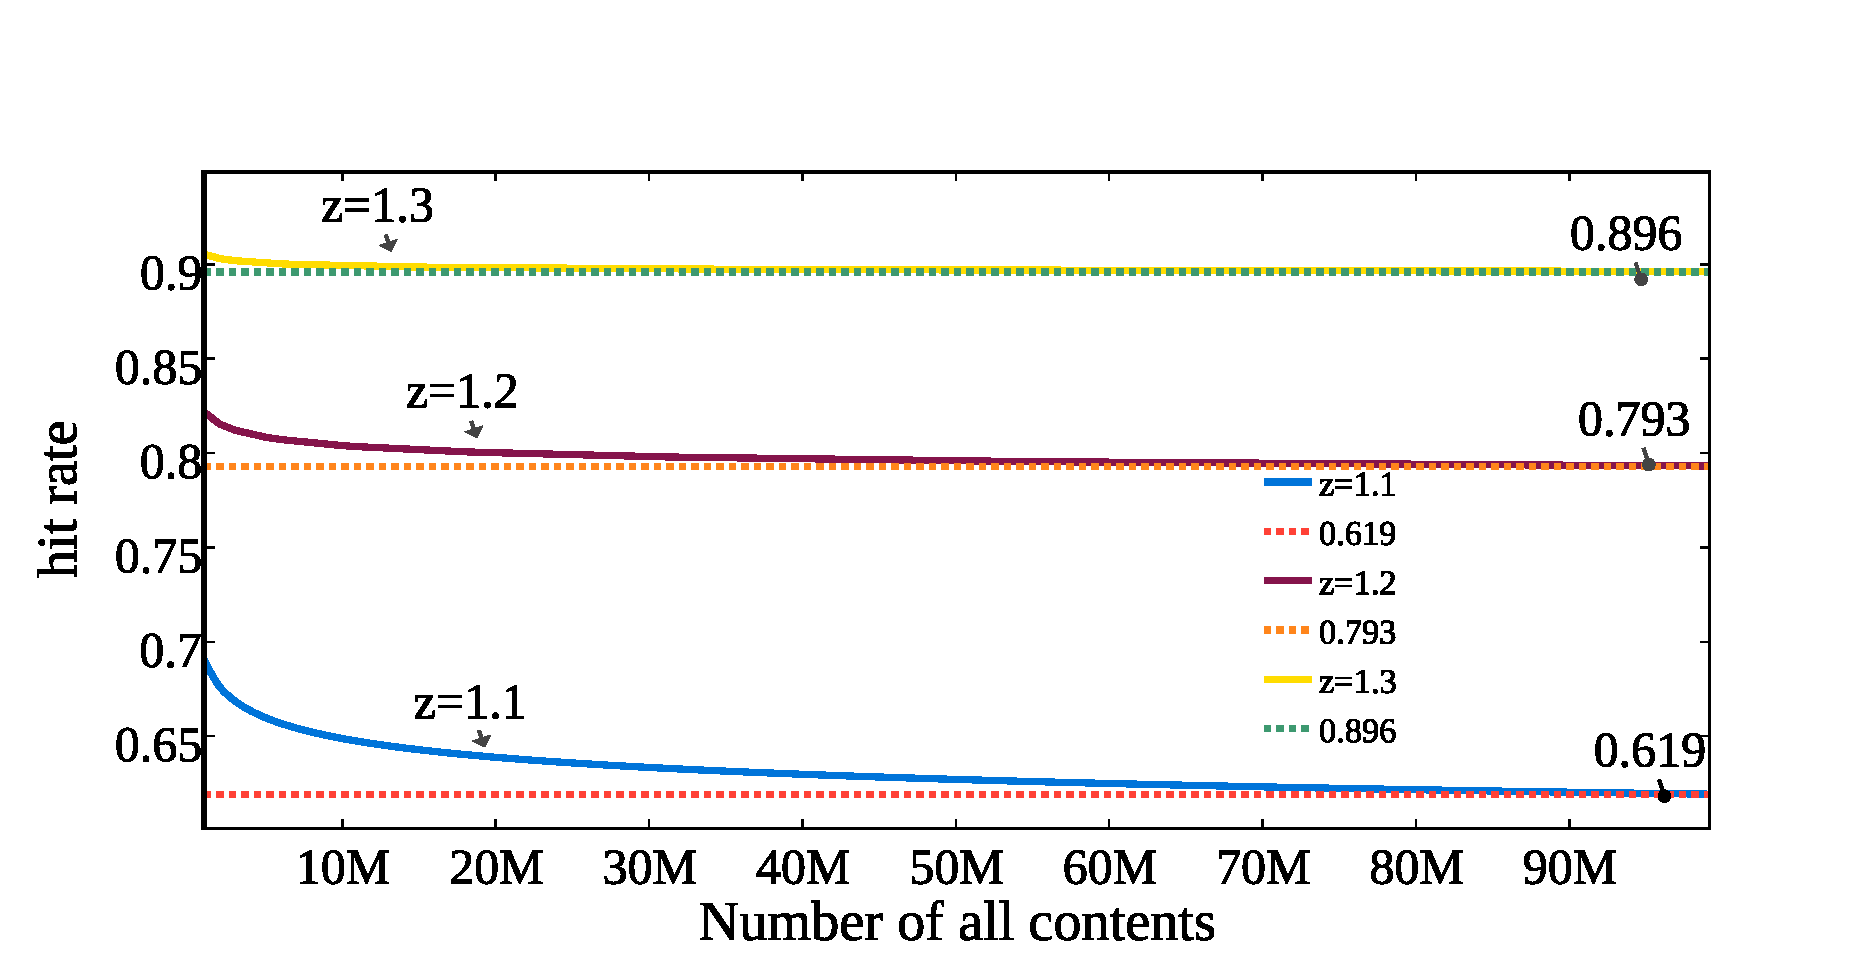
\includegraphics[width=8.8cm]{figure/hitrate.eps}
%%\caption{theoretical hit rate convergence curve, cache size:1000}
%%\label{Fig.2}
%%\end{figure}
%This is the preconditions for the feasibility of our big data reference architecture.
%
%The generic term satisfaction can be interpreted in different ways, where a natural interpretation would be obtaining a high quality of service (QoS) for the lowest price. One can not neglect the importance of \emph{cost} in user experience, in this paper, as a term of \emph{cost} on the user side, we take user's \emph{energy cost} as a \emph{service price}, for a more accurate description, to address the issue of user experience, we capture the user satisfaction or user experience using a utility function\cite{khan2011user}, the term utility comes from the field of Economics.

For evaluating system performance, we define aggregate throughput of the converged network as:
 \begin{dmath}
  TH=TH_b+TH_c\\
    =TH_{b}+\sum_i^N{TH_{ci}}\\
    =N_b\zeta_0+\sum_i^N{(1-r_i)\lambda_i\zeta_0}\\
  \end{dmath}
 where $TH_b$ is throughput of all contents which is pushed in broadcast, and $TH_{ci}$ is the user $i$'s cellular network throughput.
 
 Therefore, the Throughput Efficiency is: 
 \begin{dmath}
    \eta=\frac{\textit {effective throughput} }{\textit {aggregate throughput} }\\
    =\frac{\sum_i^N{\lambda_i\zeta_0}}{TH}\\
    =\frac{\sum_i^N{\lambda_i\zeta_0}}{N_b\zeta_0+\sum_i^N{(1-r_i)\lambda_i\zeta_0}}\\
    \label{eq:th}
  \end{dmath}
  
And as discussed in section II.B, the equivalent network capacity is:
 \begin{dmath}
\sum_{i=1}^N {B_{csi}B_{cei}} + r_i\lambda_i B_bB_{be}
    \label{eq:ec}
  \end{dmath}
  
  For simplicity, we ignore the difference of cellular subchannel bandwidth of each user, so the problem can be written as:
     \begin{dmath}
\max  N{B_{cs}B_{ce}} +  \sum_{i=1}^N r_i\lambda_i B_bB_{be}
    \label{eq:ec}
  \end{dmath}
  
 Subject to
   
 \begin{dmath}
 r_i=\sum_{n=1}^{\xi_i} f(j;z;n)
 \end{dmath}
 
Considering that our work is based on a converged broadcast and cellular networks, for evaluate the user experience, it is necessary to point out the difference of power consumption between broadcast and cellular networks.

%For simplicity, in cellular network, the SINR is given by:
%\begin{equation}\label{c_SINR}
%\begin{aligned}
%\gamma _{ci}=\frac{p_{ci}g_{ci}}{\sum_{k=0,k\not =i}^{N}{p_{ck}g_{ck}} +\sigma ^2}
%\end{aligned}
%\end{equation}
%
%Similarly, in the broadcast network, the SINR is :
%\begin{equation}\label{b_SINR}
%\begin{aligned}
%\gamma _{bi}=\frac{p_{bi}g_{bi}}{\sigma ^2}
%\end{aligned}
%\end{equation}
%
%based on shannon theorem, cellular transfer rate:
%\begin{equation}\label{c_tr}
%\begin{aligned}
%tr_c=\log_2(1+\frac{\mid g_{ci} \mid^2p_{ci}}{\sigma ^2} )
%\end{aligned}
%\end{equation}
%
%broadcast transfer rate:
%\begin{equation}\label{b_tr}
%\begin{aligned}
%tr_b=\log_2(1+\frac{\mid g_{bi} \mid^2p_{bi}}{\sigma ^2} )
%\end{aligned}
%\end{equation}
%
%now we define a user utility function:
%\begin{dmath}
% u(p_{ci},p_{bi},\pi _i)=
% \frac{L_cR_c}{M_cp_{ci}}f(\gamma _{ci})-(1-\pi_i)\frac{L_bR_b}{M_bp_{bi}}f(\gamma _{bi})+\pi_i\frac{L_bR_b}{M_bp_{bi}}f(\gamma _{bi})
%   =\frac{L_cR_c}{M_cp_{ci}}f(\gamma _{ci})+(2\pi_i-1)\frac{L_bR_b}{M_bp_{bi}}f(\gamma _{bi})
%\end{dmath}
%where 
%\begin{dmath}
%f(\gamma _i)=[1-exp(-0.5\gamma _i)]^M
%\end{dmath}


For simplicity, let the UE's power consumption of a request for cellular network given by $p_c$, and the power consumption of pre-caching a broadcast content item is $p_b$, then for the user $i$, its power consumption can be given by:
\begin{dmath}
P_i(\xi_i,r_i)=p_b\xi_i+ \lambda_i(1-r_i)p_c
\end{dmath}

Minimizing the power consumption of all users can be described as:
\begin{dmath}
 \min \sum_{i=1}^{N} (P_i(\xi_i,r_i))=
 \min \sum_{i=1}^{N}(p_b\xi_i+ \lambda_i(1-r_i)p_c)\\
 \end{dmath}

 Subject to
 \begin{dmath}
 r_i=\sum_{n=1}^{\xi_i} f(j;z;n)
 \end{dmath}

It is an optimization problem, the hit rate has close relationship with the cache size, and the related replacement algorithm. Considering the difference of user behavior, the $\lambda_i$ follows a normal distribution. In next section, based on our push scheme, we will get a simulation-based conclusion.  
 
The algorithms we will introduce focus on two main processes: pushing process and caching process. In the pushing process, our goal is to cut down the deadweight loss of energy consumption by UE adaptively adjustment. In the cache process, we develop the algorithms to increase the hit rate so that improve the system performance. In the following we will describe these two processes in details.    
 
  
\subsection{Cache Replacement Algorithm to Improve capacity:}
Before we introduce the pushing process, it is necessary to introduce the related caching process, there is a rich body of the existing papers on several aspects of  caching strategy including object replacements, cooperation cache in traditional wired networks\cite{kumar2014cache}, the scenario this paper explored is mainly based on cellular network,
in which the nodes are mainly mobile equipment, therefore it is different from wired networks in physical layer or other upper layer like application layer. As a result, the available cache solutions in existing wired network are not directly applicable for the proposed converged architecture.
        
Most of the cache strategies are based on two key dimensions: \emph{recency} and \emph{frequency}, in this paper, we focus on the popularity of each requested content, the  \emph{frequency} could well represent the \emph{popularity}. In addition, Another significant feature of popular contents is timeliness, this falls under the category of \emph{recency}. 
LRU (Least Recently Used) and LFU (Least Frequently Used)  are two typical cache replacement policy, respectively. 
As we talk about \emph{popular contents}, both of  the requesting frequency and contents timeliness should be concerned about. And because of this, in this  paper, we adopt two UE-based LRU and LFU algorithms based on our converged network architecture, which are given in Algorithm \ref{alg:cr}.
\begin{algorithm}
\caption{ Related cache replacement algorithm}
\label{alg:cr}
\begin{algorithmic}[1]
\Procedure{UE-based LRU} {}
\For{each request}
\If{$ \exists i:cache[i] == \textit{requested content}$}
\State $cache[i].count = 0 $
%\Comment higher the count the more least recently content is requested.
\Else
\If{$\textit{cache.length}\textgreater N_b$}
\State $t = \arg \max \limits_{p} \{cache[].count\}$
\State $cache[t]\stackrel{replace}{\longleftarrow} \textit{requesting content}$

\Else
\State $cache\stackrel{add}{\longleftarrow} \textit{requesting content}$
\EndIf
\EndIf
\State \textit{increment all the counts}
\EndFor
\EndProcedure
\Procedure{UE-based LFU} {}
\For{each request}
\If{$ \exists i:cache[i] == \textit{requested content}$}
\State $cache[i].count += 1 $
%\Comment higher the count the more least recently content is requested.
\Else
\If{$\textit{cache.length}\textgreater N_b$}
\State $t = \arg \min \limits_{p} \{cache[].count\}$
\State $cache[t]\stackrel{replace}{\longleftarrow} \textit{requesting content}$

\Else
\State $cache\stackrel{add}{\longleftarrow} \textit{requesting content}$
\EndIf
\EndIf
\EndFor
\EndProcedure
\end{algorithmic}
\end{algorithm}

\begin{figure}[!h]
\subfigure[Hit Rate vs Cache Size]{
\centering
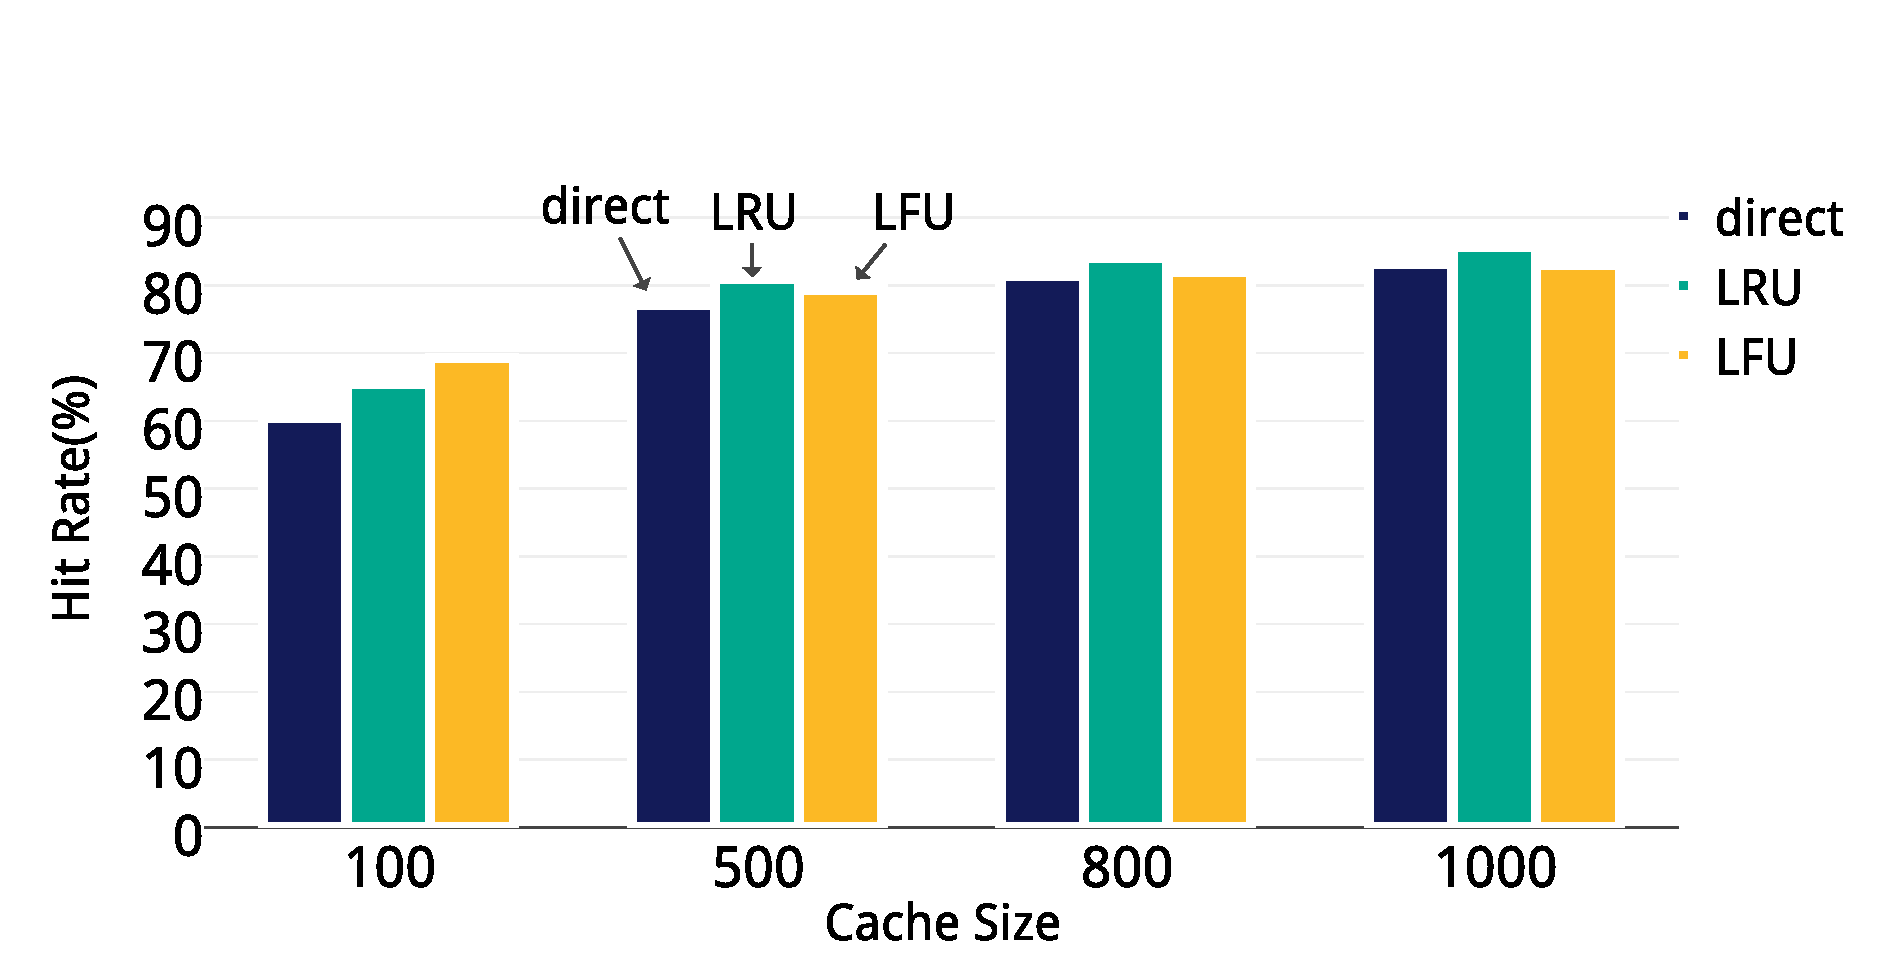
\includegraphics[width=8.8cm]{figure/hrcs.eps}
 }
\subfigure[Hit Rate vs Zipf Factor]{
\centering
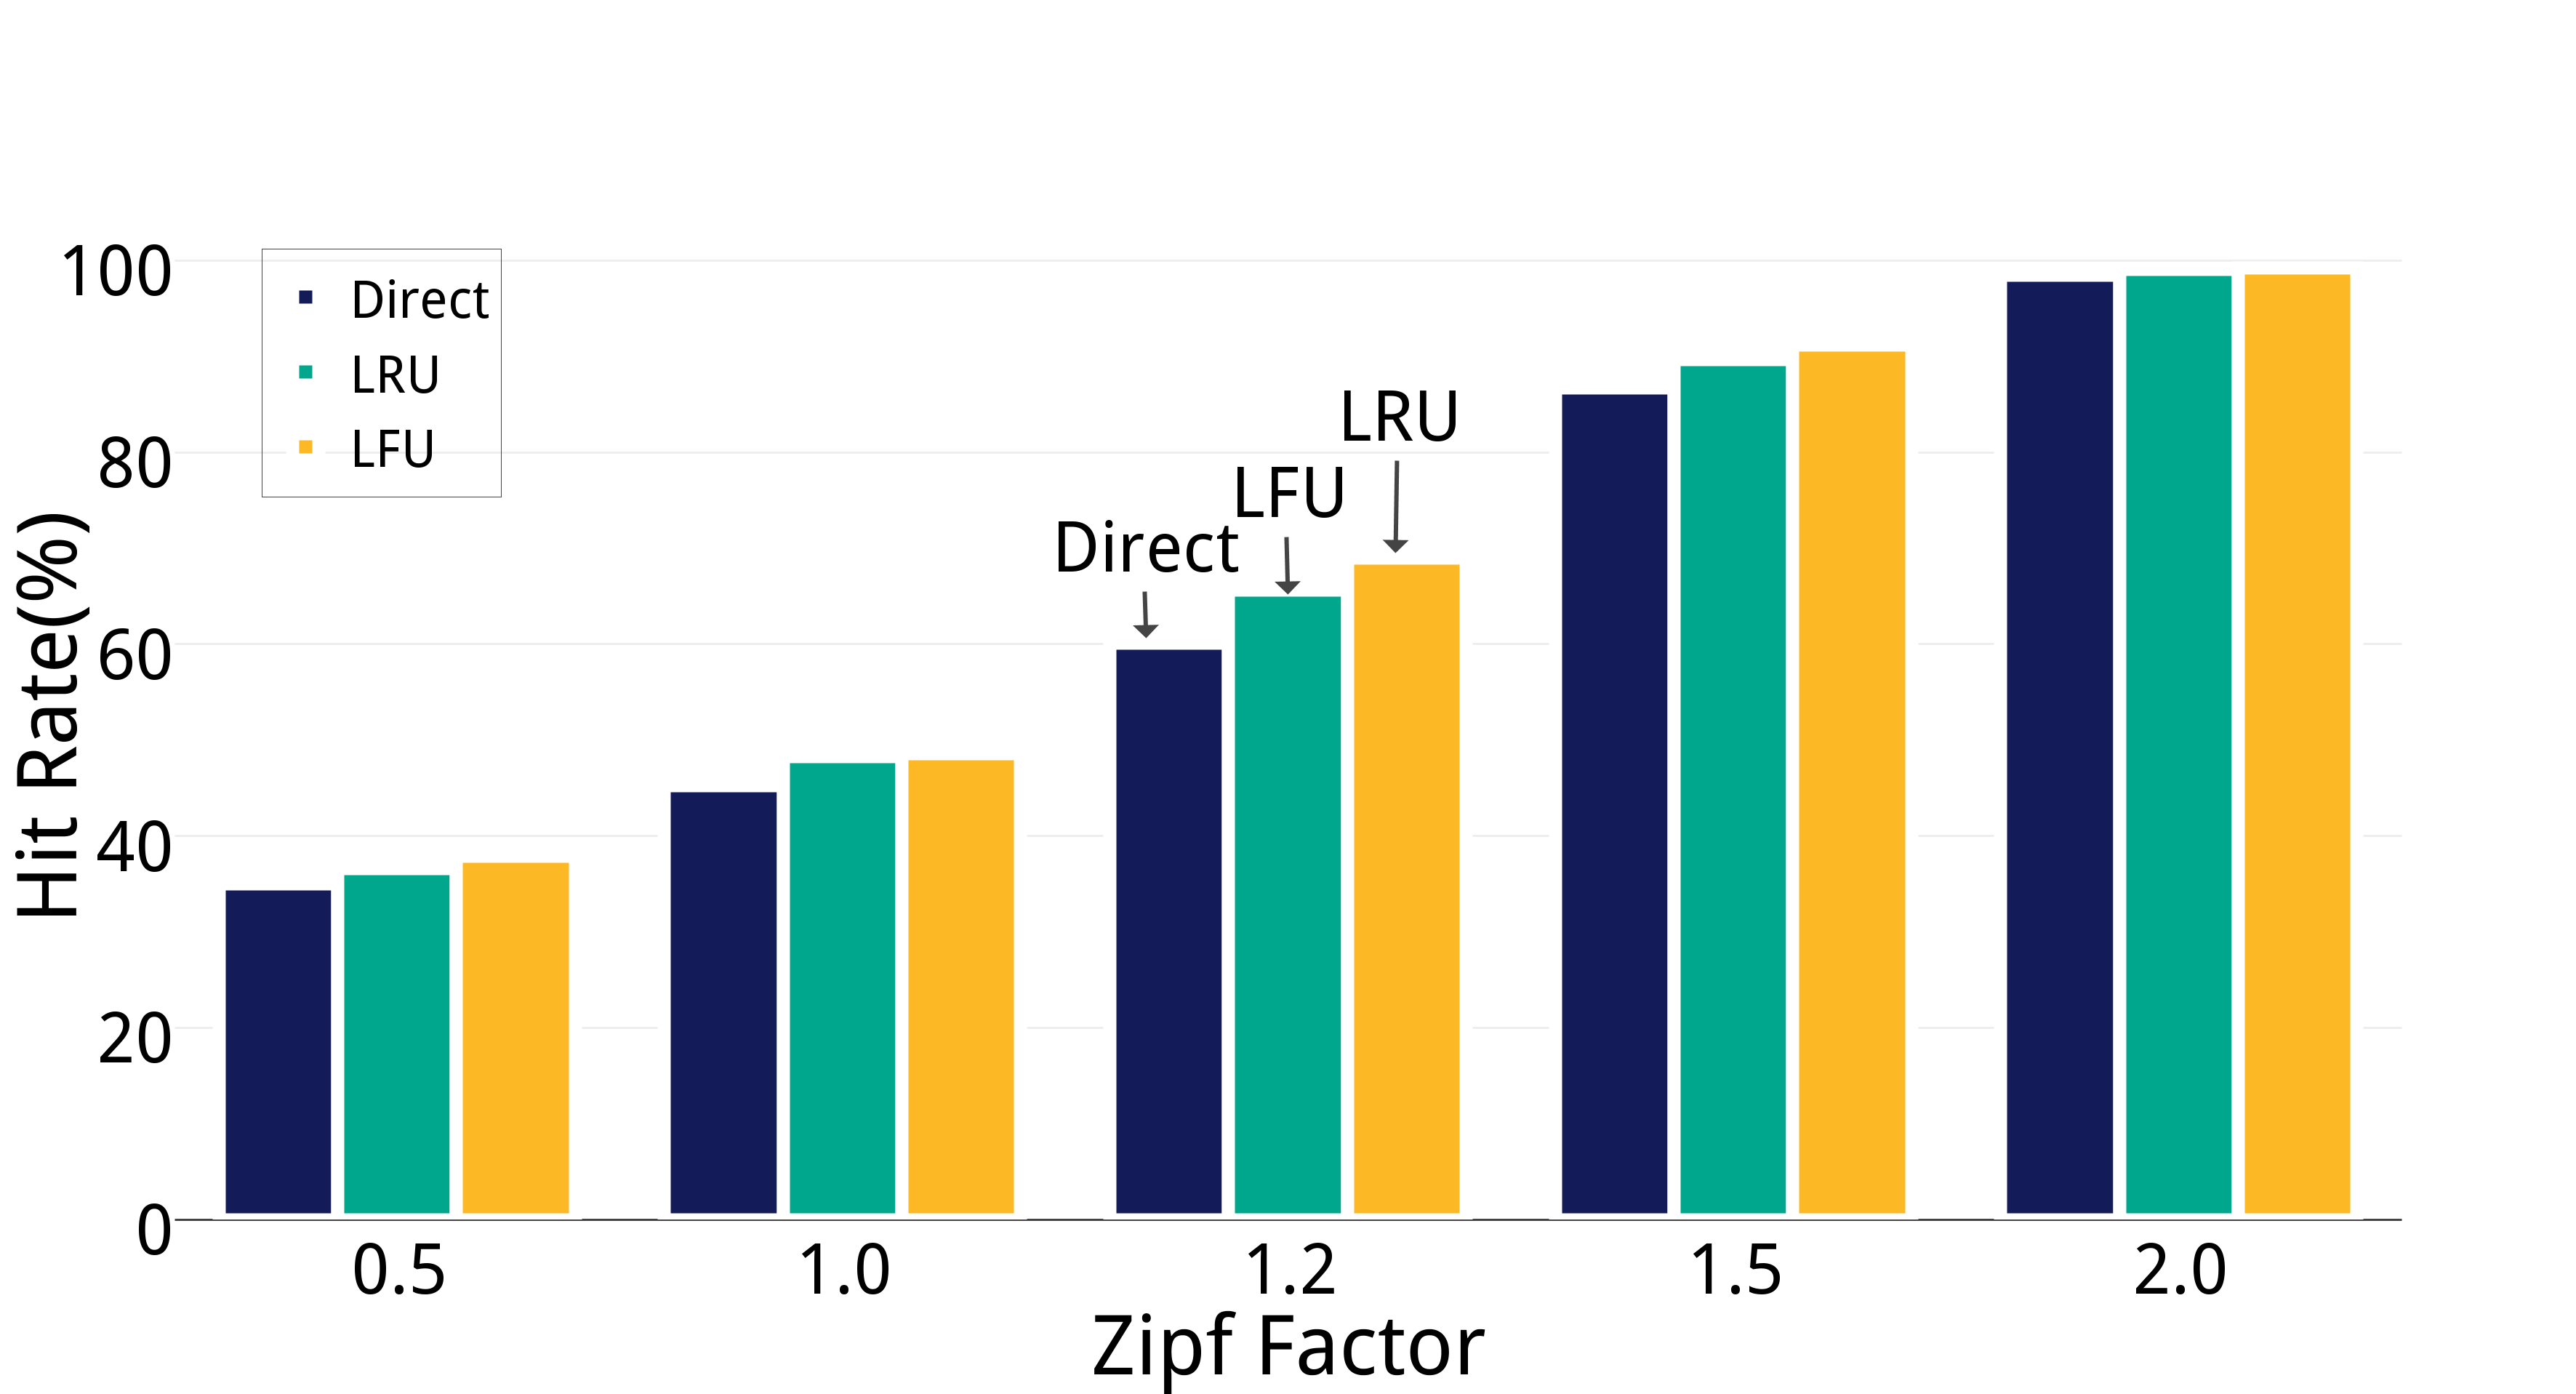
\includegraphics[width=8.8cm]{figure/hrzf.png}
}
 \caption{Hit Rate simulation}
\label{Fig.3}
\end{figure}

 \subsection{Pushing Strategy to Save Energy:}
While in the real-world situation, not every UE is interested in these popular contents, in terms of this paper, as we mentioned above, every UE has its unique hit rate because of personalization, under this situation, for these UEs, pushing and forward caching those unwanted contents would significantly increase the cost of energy and network load.
To meet the challenges, in this paper, we are interested in an asynchronous sleep-awake scheduling strategy, the main steps of the strategy are presented in Algorithm \ref{alg:sa}. In this strategy, each UE wakes up independently depends on its own \emph{cache hit rate} and \emph{request rate} in order to enhance user experience. That is, when the UE's cache mechanism is in a low hit rate or a low request rate, it falls into a sleep state, it closes the broadcast channel to avoid caching unwanted contents, with the help of this, the energy consumption of UEs is effectively reduced. At the same time, the cache mechanism is listening on the hit rate and request rate, once exceeding a threshold value, the UE turns to an awake state. In this state, the UE opens the broadcast channel and start caching the popular services being pushed. 

\begin{algorithm}[!ht]
\caption{proposed sleep-awake scheme}
\label{alg:sa}
\begin{algorithmic}[1]
\Procedure{request-response} {}
\For{each request from user $i$ \Pisymbol{psy}{206} $N$ }
	\If{$ \exists i:ServerCache[i] == \textit{requested content}$}
	\State $UserTable[i].HitCount ++$
	\EndIf
	
       \If{  $UserTable[i].HitCount \textgreater PushThreshold$ }
       \State $response.add[PushMode] = Awake$
    \For{each pushed content}
       \If{$\textit{content in local cache}$}
       	\State \textbf{Continue}
       \Else
        \State fetching and caching
        \EndIf
       \EndFor
       \Else
       \State $response.add[PushMode] = sleep$
        
    \EndIf
   

\EndFor
\EndProcedure
\end{algorithmic}
\end{algorithm}


\section{Simulation and analysis}

\begin{table}[hbt]
\footnotesize
\renewcommand\arraystretch{1}
\begin{center}
\caption{\label{Table2}Simulation Parameters}
\begin{tabular}{c|c}
\toprule
\hline
 Parameter  &    Values \\
  \hline
 Num. of users  & $N=30$ \\
   Cache Size &cache = [100,1000)   \\
  zipf factor & $\alpha=0.5,1,1.2,1.5 $   \\
    Max. Num. of push contents &   $N_b=1e3$  \\
    \hline
\bottomrule
\end{tabular}
\end{center}
\end{table}
%First step of our simulation is to theoretically verify if the hit rate is convergent as the number of contents increasing under the zipf requesting model. From Fig \ref{Fig.2} we can see that as the number of contents increases the hit rate tends to be stable, this provides the prerequisites for the simulation and research in this paper. 



\begin{figure}[!h]
\centering
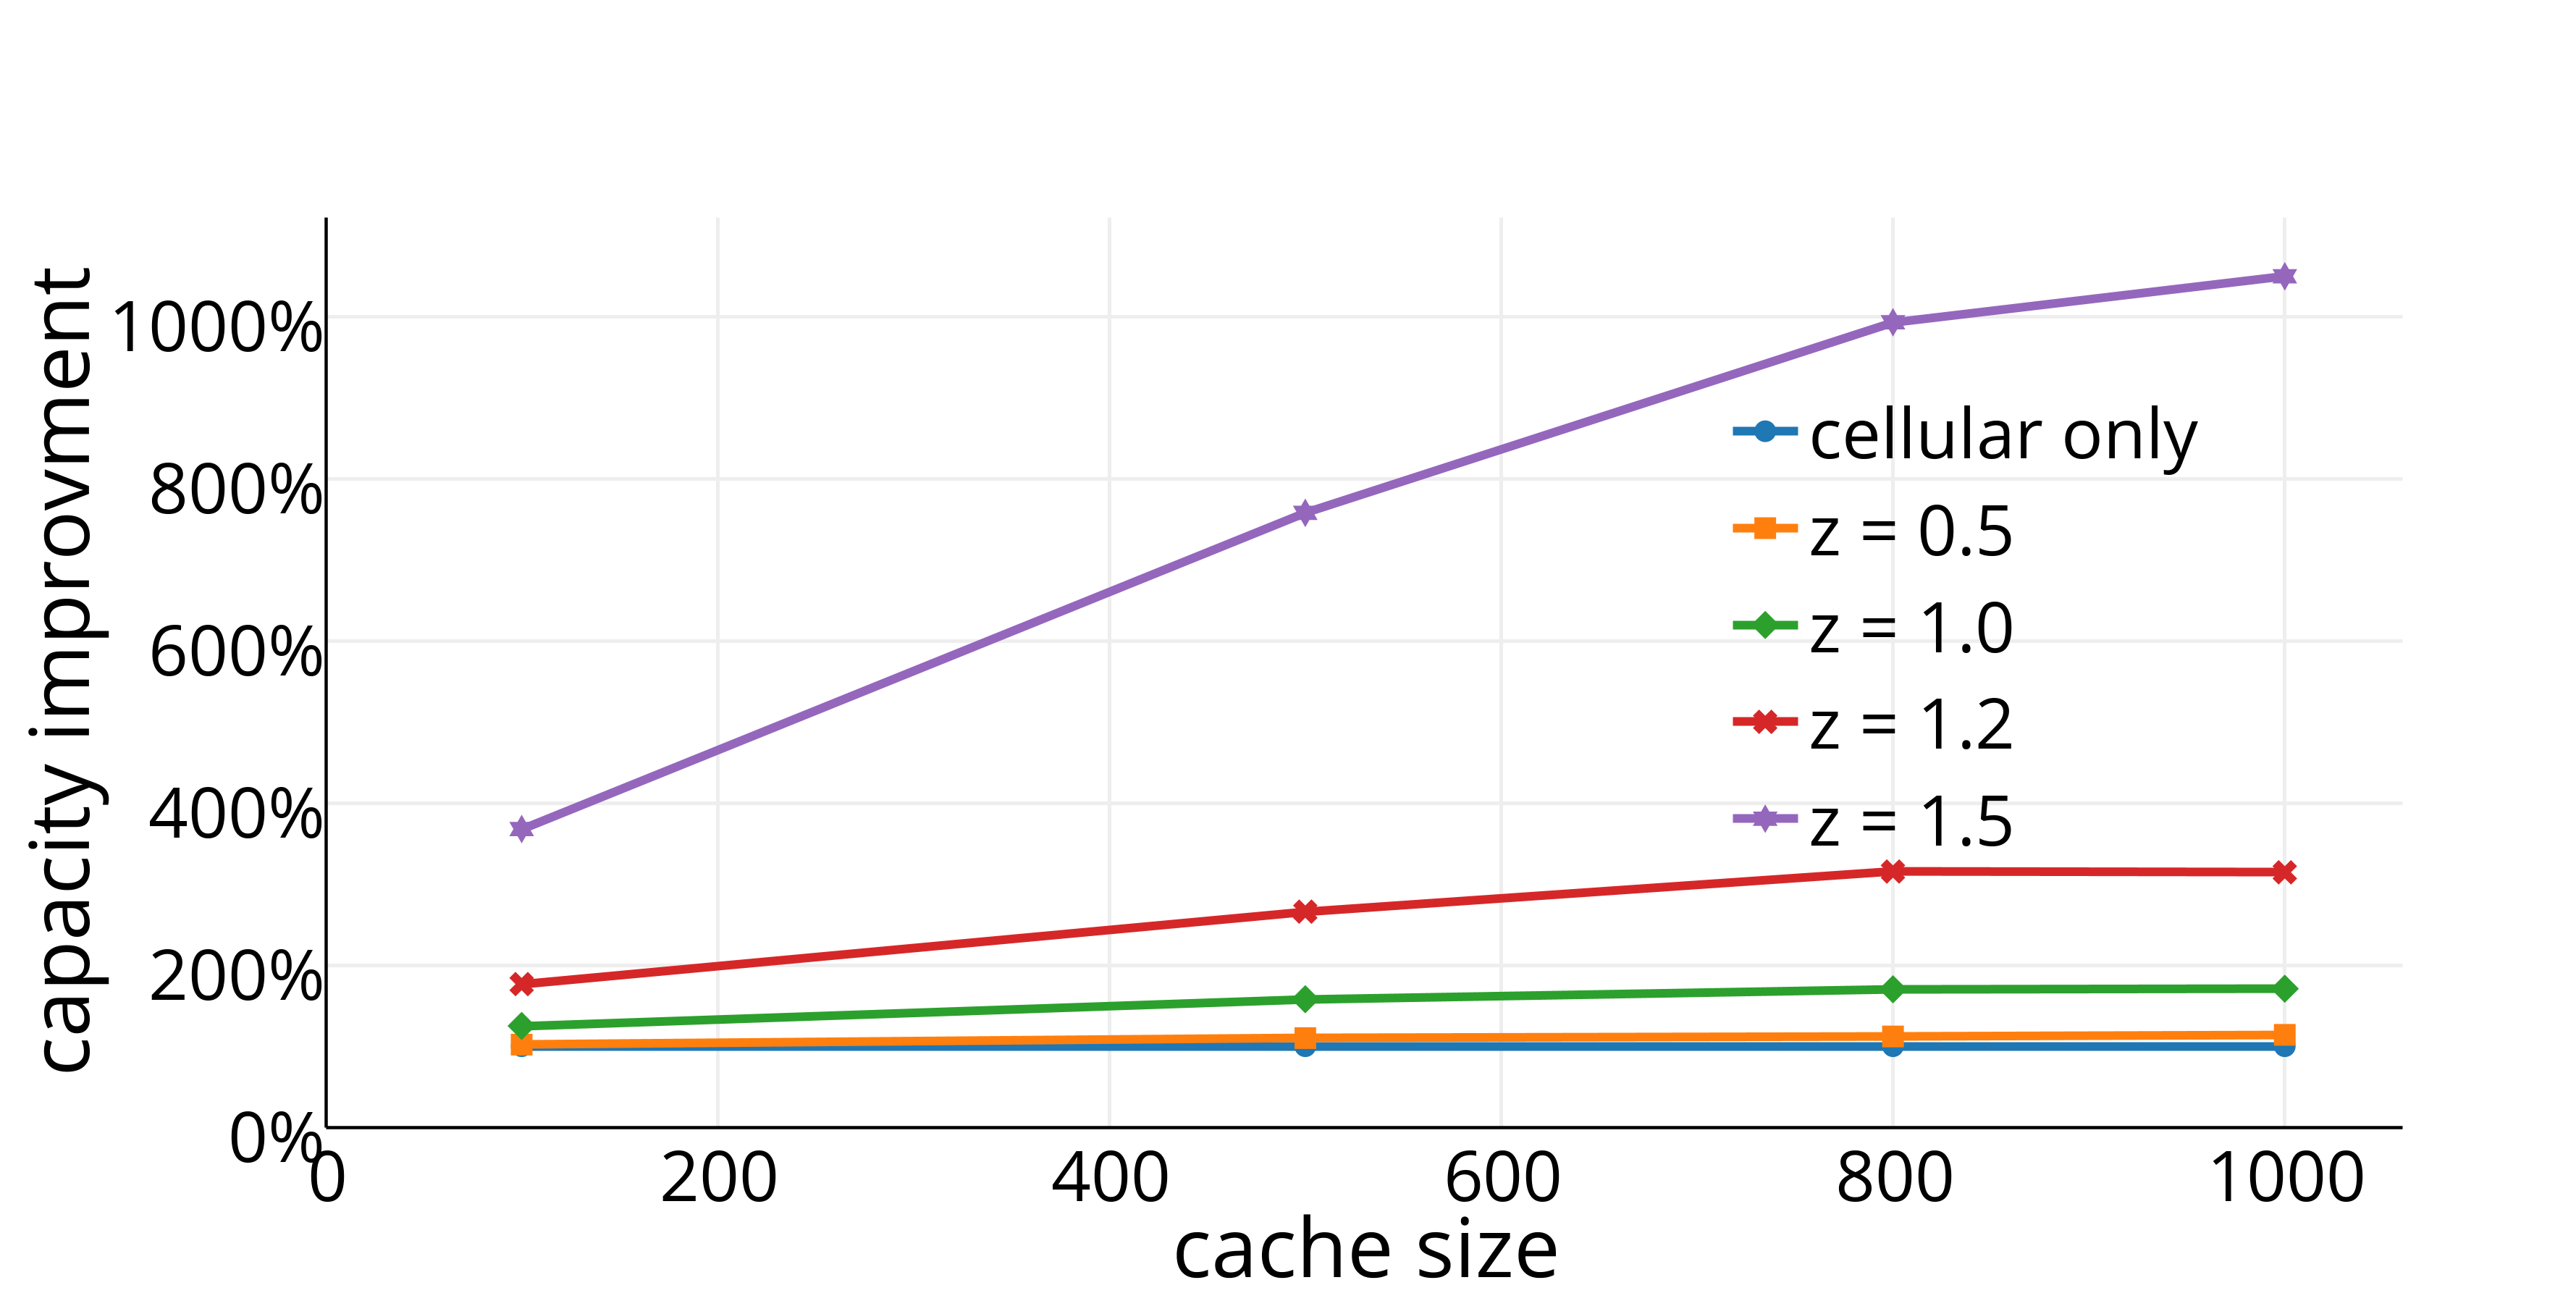
\includegraphics[width=8.8cm]{figure/capacity-new.png}
 \caption{Capacity improvement comparison by the proposed scheme}
\label{Fig.4}
\end{figure}

%\begin{figure}[!h]
%\centering
%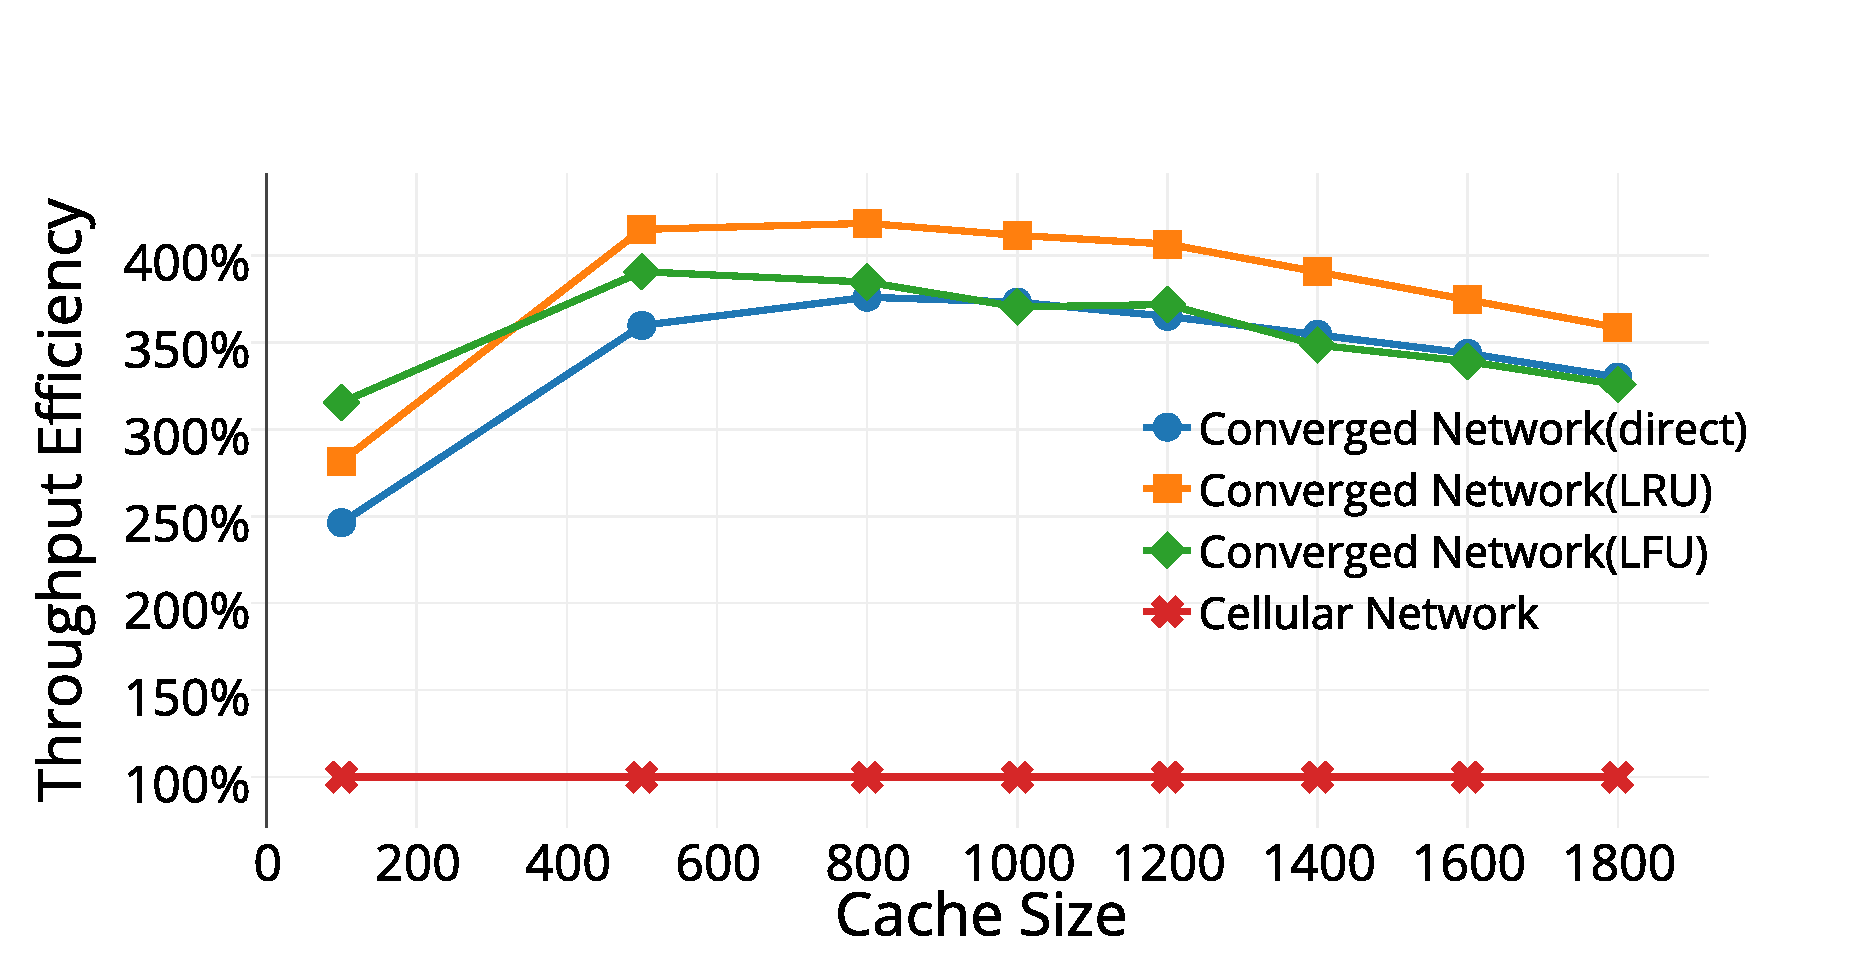
\includegraphics[width=8.8cm]{figure/efficiency.eps}
% \caption{throughput efficiency}
%\label{Fig.5}
%\end{figure}

We simulated the performance of UE's local cache hit rate of the \emph{LRU} and \emph{LFU} cache replace algorithm, for comparison, we also analyzed \emph{direct replace algorithm}, which means cache directly replace the exists one when cache is full. The related parameters are given in the Table \ref{Table2}, The numeric simulation result shows in Fig \ref{Fig.3}. The results show that with proper cache replacement algorithms the UEs' cache efficiency is increased, and makes it a non real time solution, not just applicable with real time scenario like live video.  Accordingly the capacity of converged network is further improved compared with the traditional one.

Although the proposed converged network architecture brings significant network capacity improvement shown in Fig \ref{Fig.4}, the inevitable cache miss events would cause the problem of efficiency, so we defined \emph{Throughput Efficiency} given in the equation \eqref{eq:th}, from the simulation results, we can find a maximum point between 500 to 800(cache size), indicating that the more cache or the more broadcasting is not always better. Too much caching would cause a waste of network resources, and make it lower efficient. For users, this degrades the user experience in battery consumption and storage occupancy. 

Based on this phenomenon, we simulate the proposed sleep awake strategy by examine the energy consumption. Fig \ref{Fig.ezf05} Fig \ref{Fig.ezf1}, Fig \ref{Fig.ezf12} and Fig \ref{Fig.ezf15} are the  energy consumption comparison of \emph{CN}, \emph{CBCN} and proposed sleep awake scheme in \emph{CBCN} under the conditions of different zipf factor. By comparison, the converged network turns out to be a more energy-efficient architecture. Moreover, with the proposed sleep awake pushing scheme, the three figures prove that when the cache contents size of each UE dynamically changes with the different needs, the energy consumption will get a significant improvement. 

Compared with traditional cellular network, the energy consumption of converged architecture is reduced by 60\% when the cache size is 800 and zipf factor is close to 1, which matches the practice better. 

Compared with converged network, the proposed scheme in converged architecture get a 20\% more reduction on energy consumption.



\begin{figure}[t]
\centering
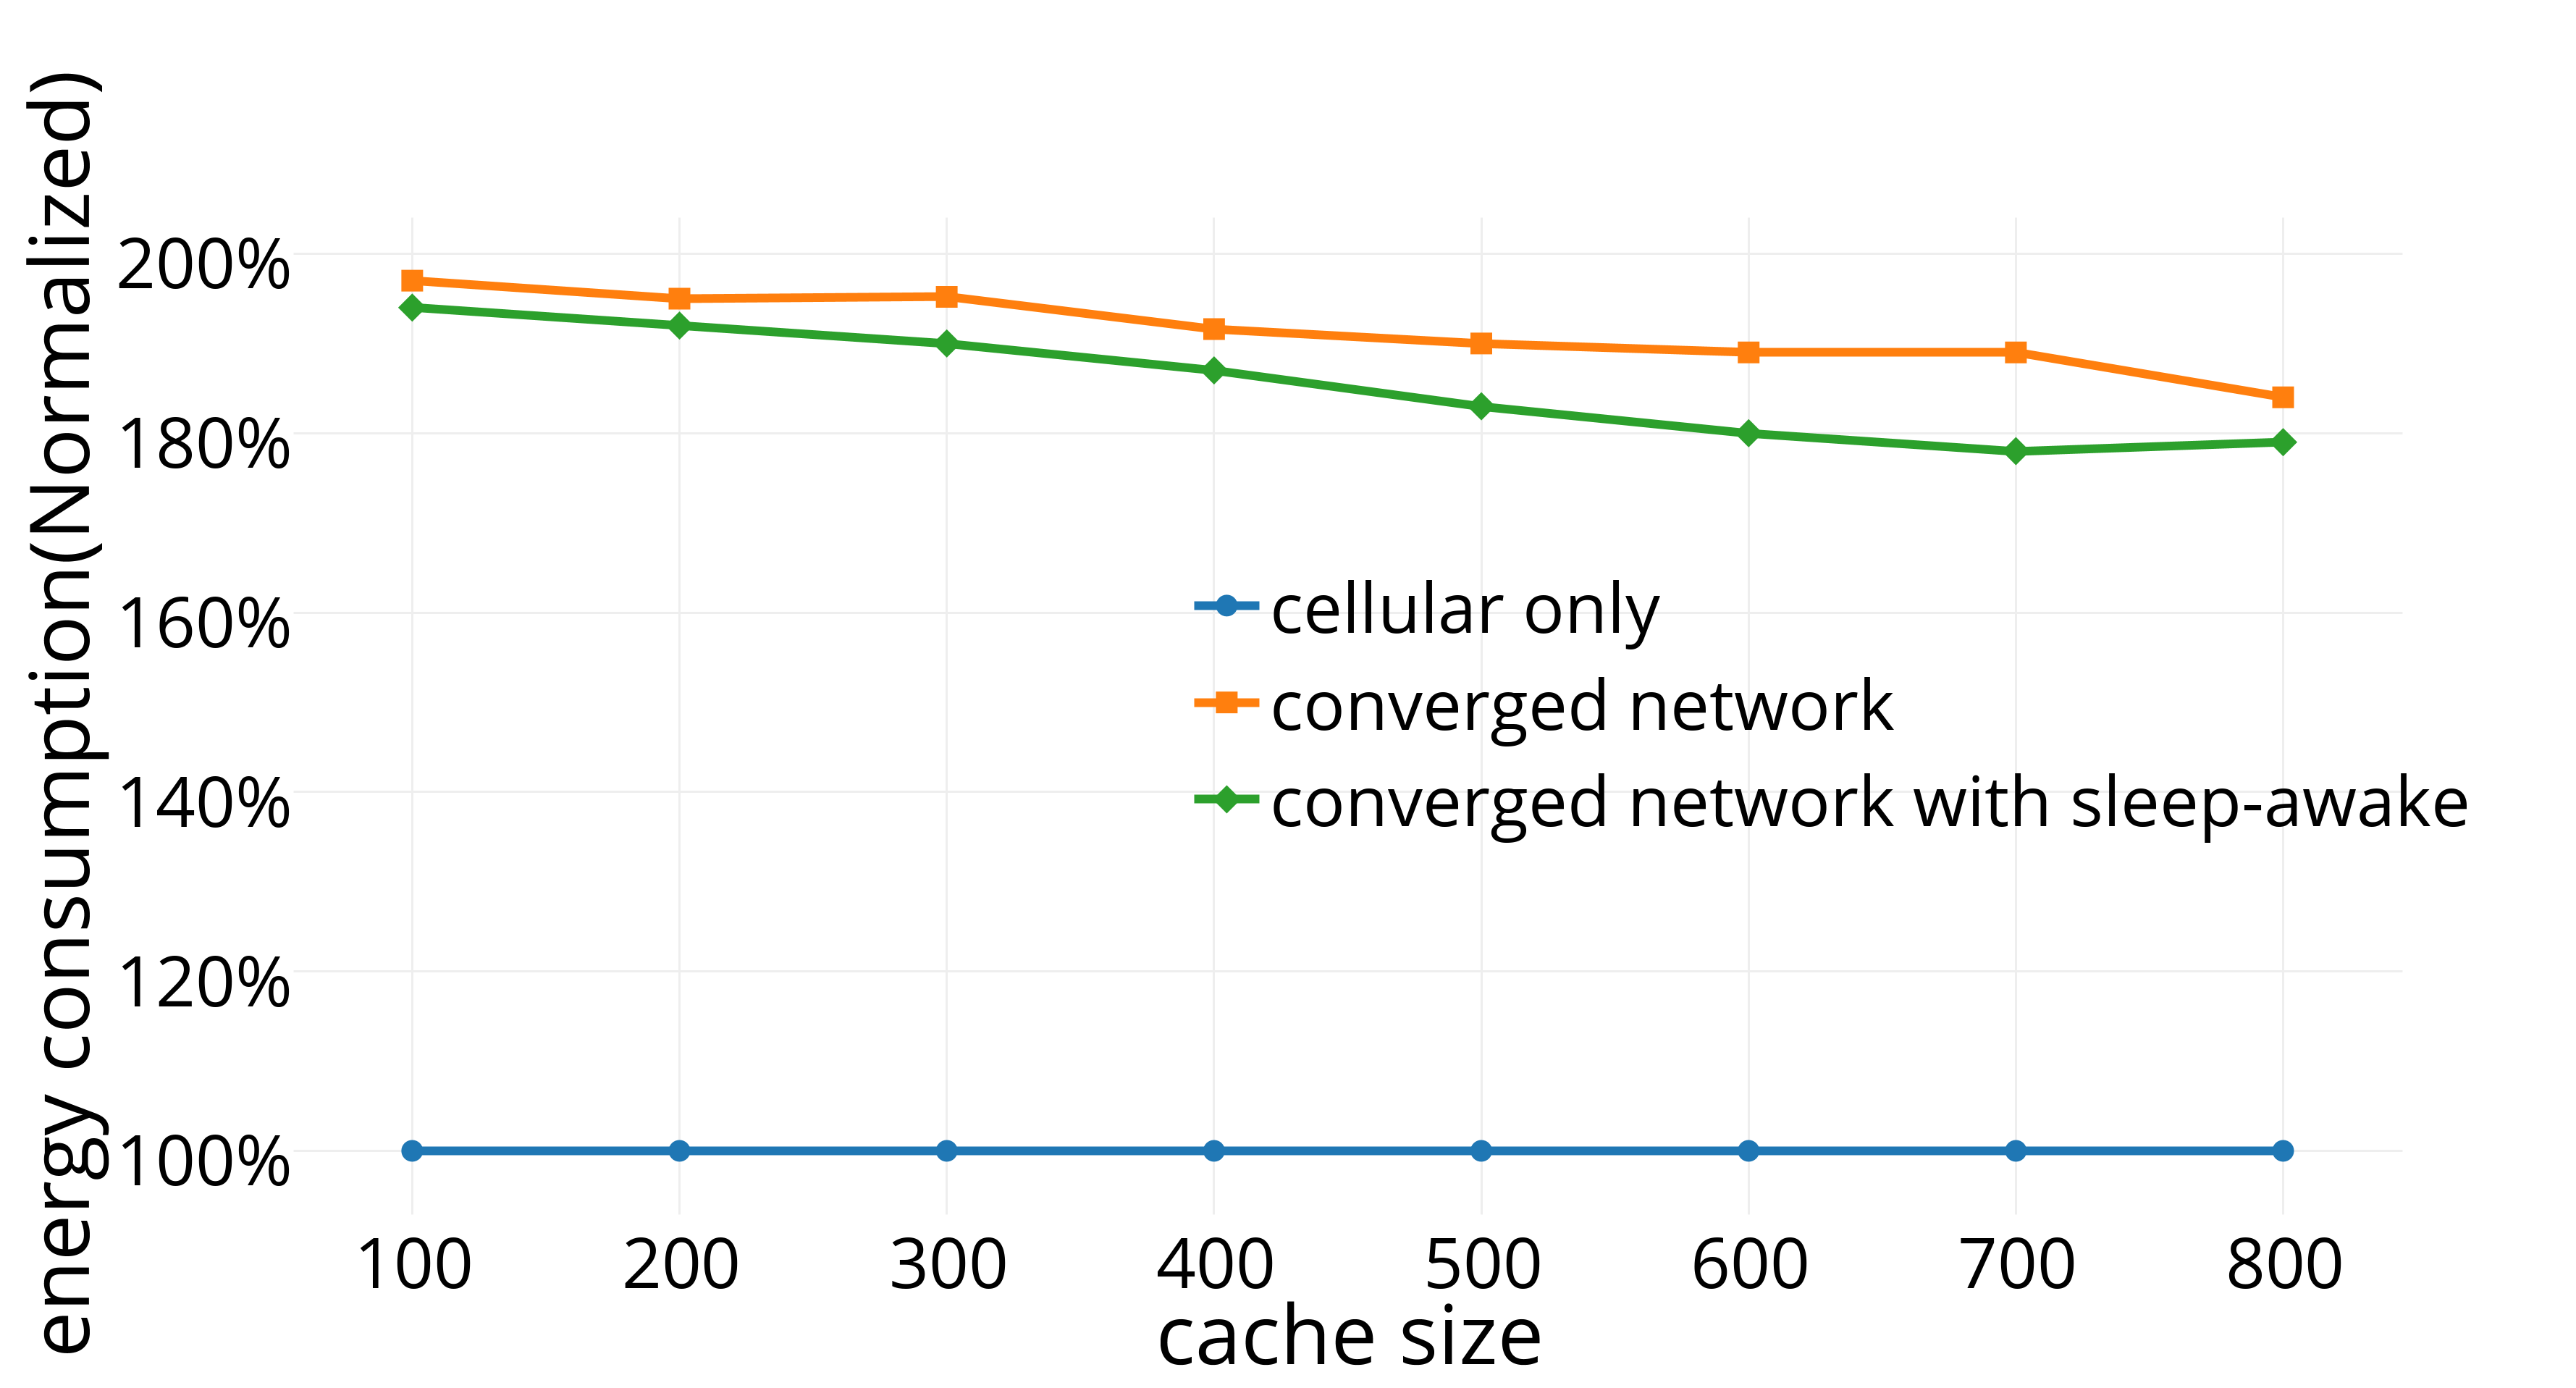
\includegraphics[width=8.8cm]{figure/energy05.png}
 \caption{Energy consumption comparison (zipf factor=0.5)}
\label{Fig.ezf05}
\end{figure}

\begin{figure}[t]
\centering
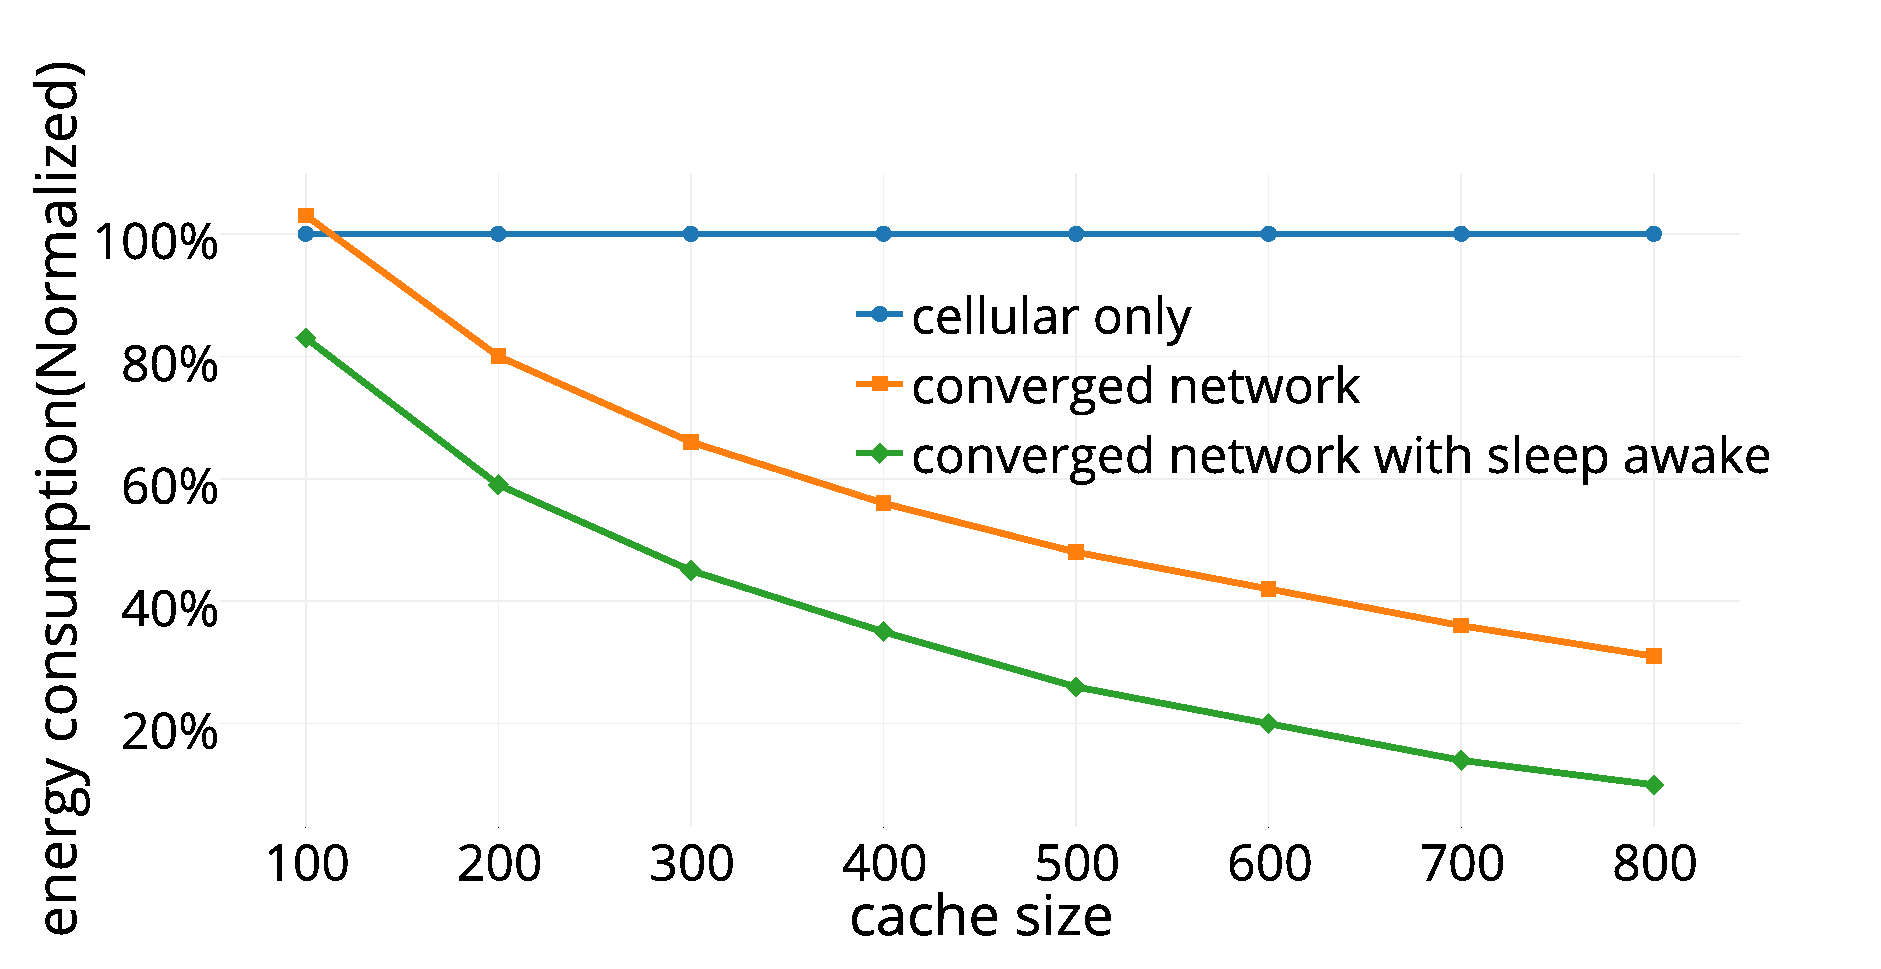
\includegraphics[width=8.8cm]{figure/energy-zipf-factor=1.eps}
 \caption{Energy consumption comparison (zipf factor=1)}
\label{Fig.ezf1}
\end{figure}


\begin{figure}[t]
\centering
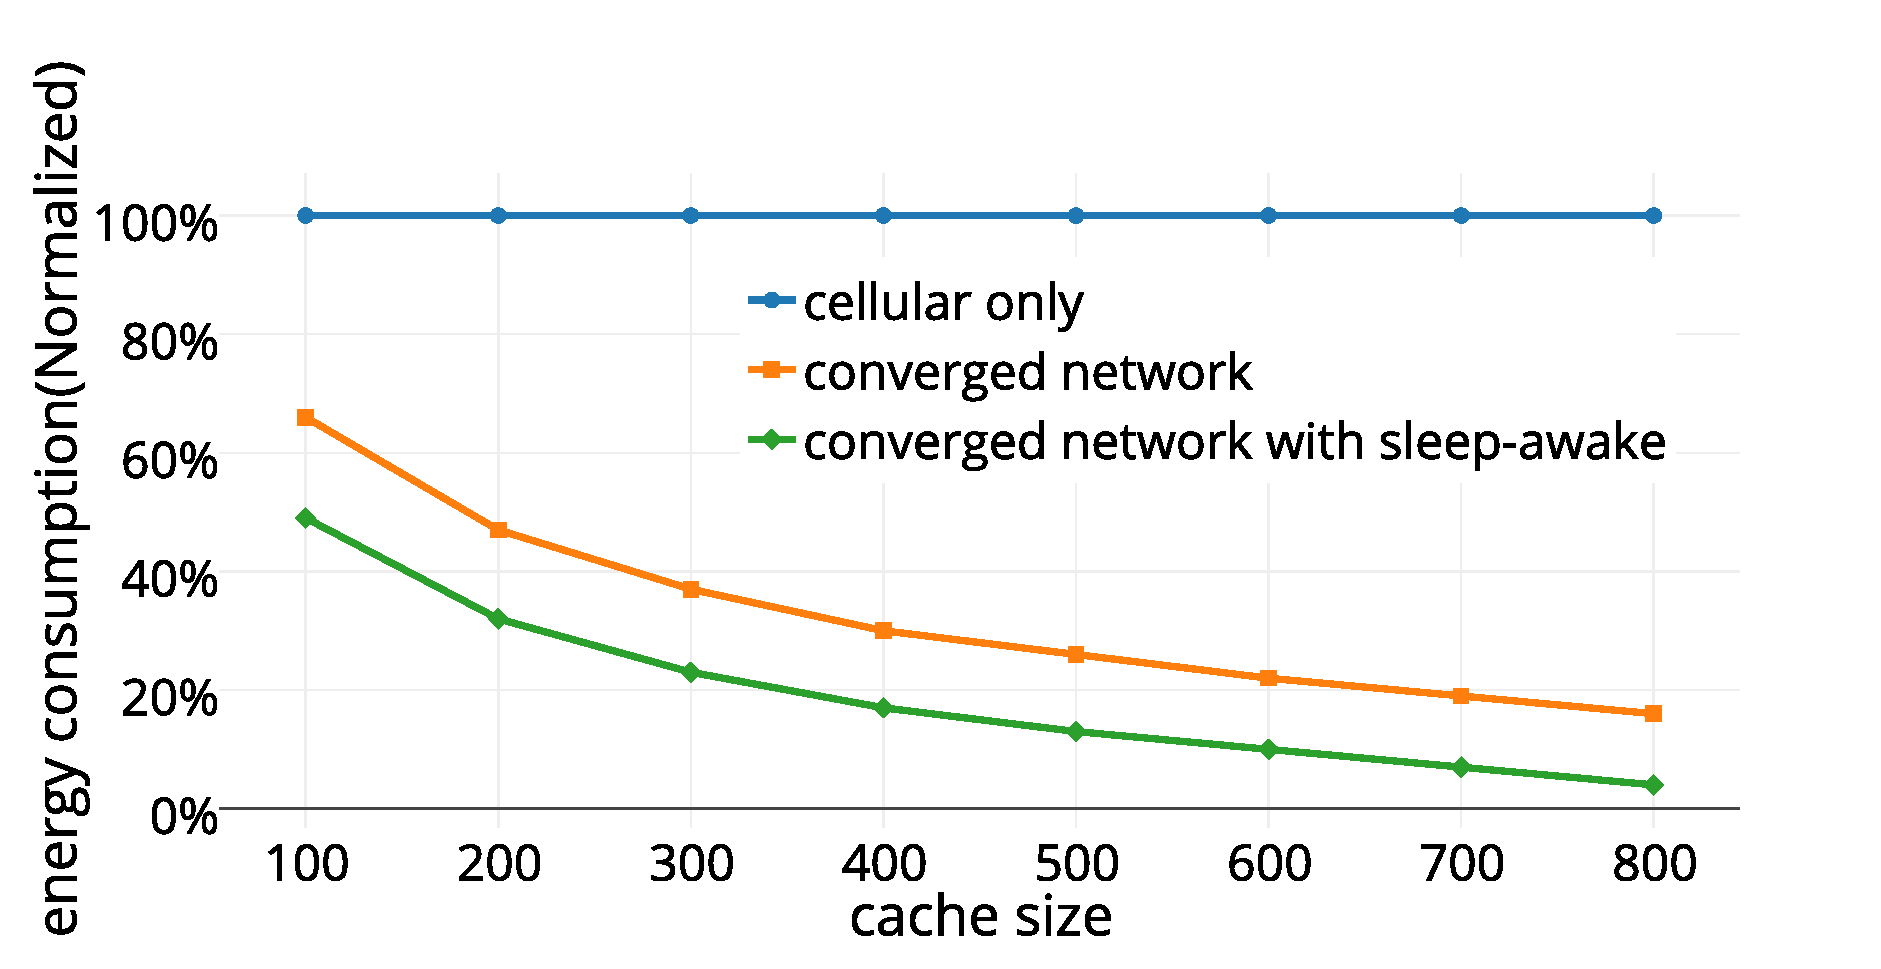
\includegraphics[width=8.8cm]{figure/energy-zipf-factor=12.eps}
 \caption{Energy consumption comparison (zipf factor=1.2)}
\label{Fig.ezf12}
\end{figure}

\begin{figure}[t]
\centering
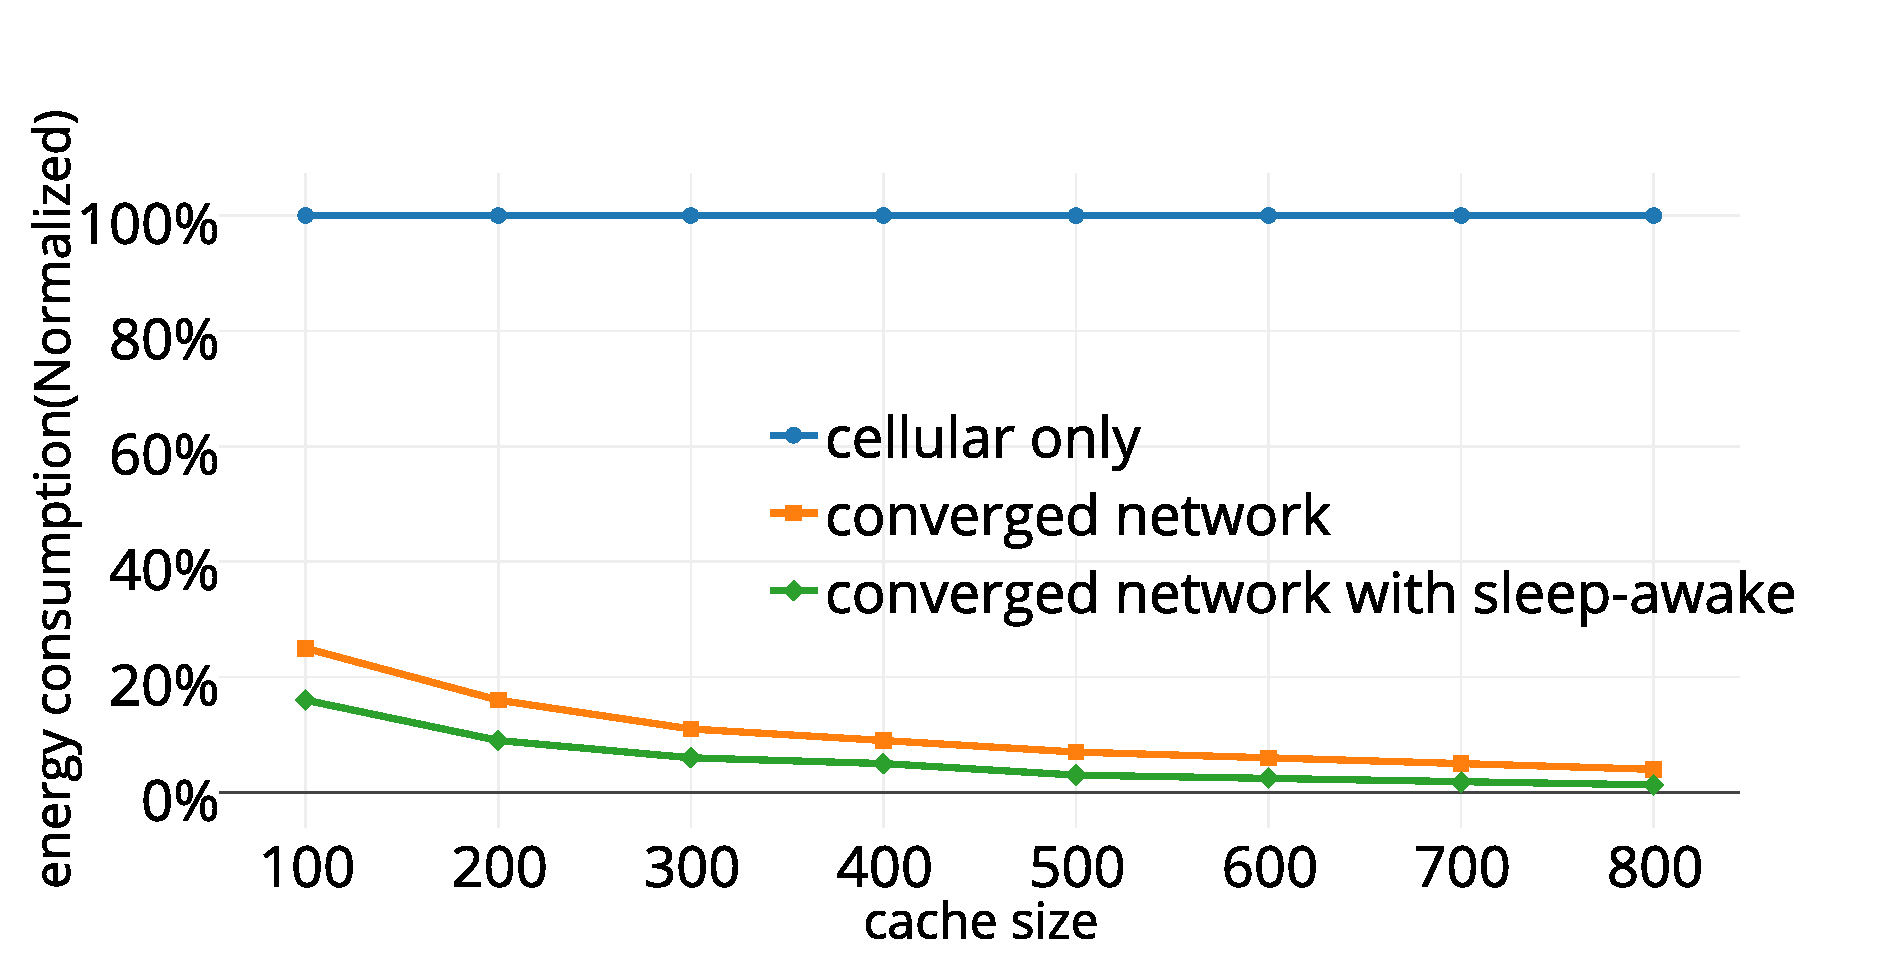
\includegraphics[width=8.8cm]{figure/energy-zipf-factor=15.eps}
 \caption{Energy consumption comparison (zipf factor=1.5)}
\label{Fig.ezf15}
\end{figure}


In summary, adopting the proposed sleep-awake pushing strategy and cache replace algorithm in our UE-based cache architecture can significantly reduce the energy consumption and improve capacity of \emph{CBCN}. If all the users has a cache and adaptively accept push services, it will save energy consumption by 20\%-30\% to the converged network. 

\section{Conclusion}
Inspired by the matthew effect of requested contents, we proposed a scheme based on push and forward cache in cellular networks. Towards this direction, we firstly introduce a related push contents cache scheme and cache replace algorithms, which makes it a non real time broadcast solution, and further improve the cache hit rate, thus improve the network capacity of our architecture. And then we suggest a sleep-awake scheme in this paper to decide the proper pushing-throughput of each user, by doing this we reduce the UEs' energy consumption. By comparing our algorithms and scheme with the traditional cellular network and converged network in simulations, it is clear that our scheme can get as much as 60\% reduction of energy consumption and nearly 200\%(when zipf factor is 1) in capacity improvement compared with cellular only network, and a 20\% further improvement compared with converged network. Future work includes real-time pushing scheduling in this scenario and considering more practical and more efficient cache strategy in \emph{CBCN}.


%
%\section*{Acknowledgment}
%
%
%The authors would like to thank...


\bibliographystyle{IEEEtran}
\bibliography{libing_citation}


\end{document}


